% THIS IS SIGPROC-SP.TEX - VERSION 3.1
% WORKS WITH V3.2SP OF ACM_PROC_ARTICLE-SP.CLS
% APRIL 2009
%
% It is an example file showing how to use the 'acm_proc_article-sp.cls' V3.2SP
% LaTeX2e document class file for Conference Proceedings submissions.
% ----------------------------------------------------------------------------------------------------------------
% This .tex file (and associated .cls V3.2SP) *DOES NOT* produce:
%       1) The Permission Statement
%       2) The Conference (location) Info information
%       3) The Copyright Line with ACM data
%       4) Page numbering
% ---------------------------------------------------------------------------------------------------------------
% It is an example which *does* use the .bib file (from which the .bbl file
% is produced).
% REMEMBER HOWEVER: After having produced the .bbl file,
% and prior to final submission,
% you need to 'insert'  your .bbl file into your source .tex file so as to provide
% ONE 'self-contained' source file.
%
% Questions regarding SIGS should be sent to
% Adrienne Griscti ---> griscti@acm.org
%
% Questions/suggestions regarding the guidelines, .tex and .cls files, etc. to
% Gerald Murray ---> murray@hq.acm.org
%
% For tracking purposes - this is V3.1SP - APRIL 2009

\documentclass{acm_proc_article-sp}
\usepackage{float}

\begin{document}

\raggedbottom

\title{MPI NAS Parallel Benchmarking}
\subtitle{CSC 569}

\numberofauthors{4} 
\author{
\alignauthor
Ian Dunn\\
       \affaddr{Computer Science Department}\\
       \affaddr{Cal Poly}\\
       \affaddr{San Luis Obispo, California}\\
       \email{idunn01@calpoly.edu}
\alignauthor
Toshi Kuboi\\
       \affaddr{Computer Science Department}\\
       \affaddr{Cal Poly}\\
       \affaddr{San Luis Obispo, California}\\
       \email{tkuboi@calpoly.edu}
       \and % go to new row
\alignauthor
Mitchell Rosen\\
       \affaddr{Computer Science Department}\\
       \affaddr{Cal Poly}\\
       \affaddr{San Luis Obispo, California}\\
       \email{mwrosen@calpoly.edu}
\alignauthor
Austin Wylie\\
       \affaddr{Computer Science Department}\\
       \affaddr{Cal Poly}\\
       \affaddr{San Luis Obispo, California}\\
       \email{awylie@calpoly.edu}
}

\date{13 October 2013}

\maketitle

\section{Introduction}
With the goal of exploring the performance benefits and drawbacks of distributed computing, we set up and ran various computationally-distributable benchmarks on two cluster types. A set of the Numerical Aerodynamic Simulation (NAS) Parallel Benchmarks (NPB) were run on both the machines in lab 14-302 (with 1 to 32 nodes) and Raspberry Pis (with 1 to 5 nodes). The Message Passing Interface (MPI) library was responsible for inter-machine communication. As an extra note, the lab machines have 3 GHz processors and 4 GB of memory; the Rasperry Pis have 700 MHz processors and 512 MB of memory.

Because the Pis aren't very powerful, and to directly compare the cluster types, all of our results use the class A benchmarks, which are intended to test relatively slow machines.

\section{Results}
The primary metric we explore in the benchmarks is speedup, which is calculated by dividing the time taken by the benchmark on the fewest number of nodes (usually one or two) by the time taken by the current run. We could comment on the raw runtimes of these different scenarios and the effect of different processors and RAM setups, but speedup best quantifies the improvement from actually distributing the work.

Tables~\ref{LabTable} and~\ref{PiTable} shows the NPB results for the lab machine cluster and the Pi cluster, including the specific benchmark, runtime in seconds, speedup, millions of operations per second (MOPS), and MOPS per process.

Note that not all benchmarks can use any number of processes: many require a square number or a power of two, which  is why some datapoints are absent in the following results.

In the graphs, vertical axes show the speedup and horizontal axes show the number of nodes the benchmark was run on.

%%%%% LAB MACHINES %%%%%
\subsection{Lab Machines}

%%%%% TABLE %%%%%
Table~\ref{LabTable} shows the lab machines' NPB results.

\begin{table*}[tbp]
\centering
\caption{Lab Machine Benchmark Results}
\label{LabTable}
\begin{tabular}{ c | c || c | c | c | c }
	Benchmark & Nodes & Time & Speedup & MOPS & Process MOPS\\ \hline
    BT    & 1     & 82.94 & 1.00     & 2028.91 & 2028.91 \\
    BT    & 4     & 28.19 & 2.94  & 5970.02 & 1492.51 \\
    BT    & 9     & 20.18 & 4.11  & 8337.38 & 926.38 \\
    BT    & 16    & 15.25 & 5.44  & 11037.04 & 689.82 \\
    EP    & 1     & 20.14 & 1.00     & 26.65 & 26.65 \\
    EP    & 2     & 10.11 & 1.99  & 53.09 & 26.55 \\
    EP    & 4     & 5.07  & 3.97  & 105.85 & 26.46 \\
    EP    & 8     & 2.54  & 7.93  & 211.40 & 26.43 \\
    EP    & 16    & 1.34  & 15.03 & 401.95 & 25.12 \\
    EP    & 32    & 0.64  & 31.47 & 838.80 & 26.21 \\
    FT    & 1     & 7.61  & 1.00     & 938.07 & 938.07 \\
    FT    & 2     & 6.52  & 1.17  & 1094.71 & 547.36 \\
    FT    & 4     & 7.14  & 1.07  & 999.95 & 249.99 \\
    FT    & 8     & 6.7   & 1.14  & 1065.54 & 133.19 \\
    FT    & 16    & 3.69  & 2.06  & 1936.09 & 121.01 \\
    FT    & 32    & 3.26  & 2.33  & 2186.15 & 68.32 \\
    IS    & 1     & 0.75  & 1.00     & 102.74 & 102.74 \\
    IS    & 2     & 1.18  & 0.64  & 72.30  & 36.15 \\
    IS    & 4     & 1.85  & 0.41  & 39.36 & 9.84 \\
    IS    & 8     & 2.43  & 0.31  & 37.01 & 4.63 \\
    IS    & 16    & 2     & 0.38  & 60.67 & 3.79 \\
    IS    & 32    & 4.75  & 0.16  & 53.41 & 1.67 \\
    LU    & 1     & 81.75 & 1.00     & 1459.31 & 1459.31 \\
    LU    & 2     & 43.75 & 1.87  & 2726.65 & 1363.33 \\
    LU    & 4     & 23.65 & 3.46  & 5045.09 & 1261.27 \\
    LU    & 8     & 15.81 & 5.17  & 7543.72 & 942.97 \\
    LU    & 16    & 10.17 & 8.04  & 11726.37 & 732.90 \\
    LU    & 32    & 13.52 & 6.05  & 8825.54 & 275.80 \\
    MG    & 1     & 2.65  & 1.00     & 1466.37 & 1466.37 \\
    MG    & 2     & 1.5   & 1.77  & 2598.48 & 1299.24 \\
    MG    & 4     & 1.19  & 2.23  & 3279.58 & 819.89 \\
    MG    & 8     & 1.05  & 2.52  & 3698.19 & 462.27 \\
    MG    & 16    & 0.68  & 3.9   & 5734.90 & 358.43 \\
    MG    & 32    & 0.85  & 3.12  & 4587.27 & 143.35 \\
    SP    & 1     & 95.11 & 1.00     & 893.84 & 893.84 \\
    SP    & 4     & 32.87 & 2.89  & 2586.13 & 646.53 \\
    SP    & 9     & 28.16 & 3.38  & 3019.24 & 335.47 \\
    SP    & 16    & 21.08 & 4.51  & 4033.04 & 252.07 \\
\end{tabular}
\end{table*}


%%%%% FIGURES %%%%%
Figures~\ref{LabBT} through~\ref{LabSP} graph those speedup results.

\begin{figure}[tbp]
  \centering
  \caption{BT Benchmark on Lab Machines}
	\label{LabBT}
  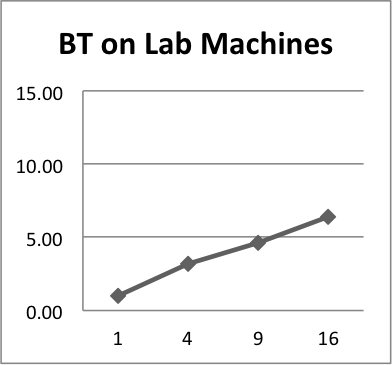
\includegraphics[width=20pc]{Pics-Lab/BT.png}
\end{figure}

\begin{figure}[tbp]
  \centering
  \caption{EP Benchmark on Lab Machines}
  \label{LabEP}
  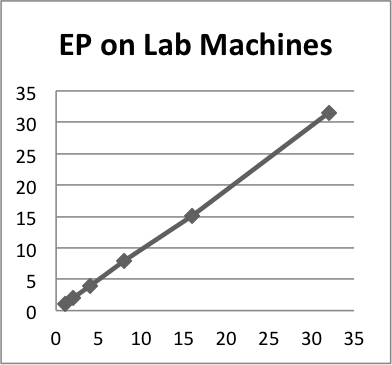
\includegraphics[width=20pc]{Pics-Lab/EP.png}
\end{figure}

\begin{figure}[tbp]
  \centering
  \caption{FT Benchmark on Lab Machines}
	\label{LabFT}
  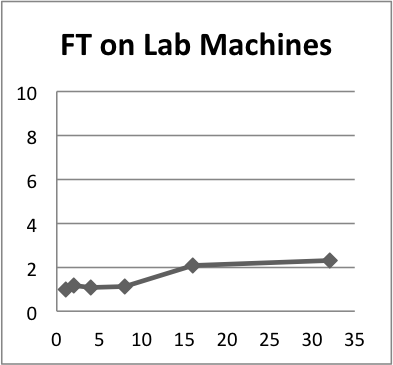
\includegraphics[width=20pc]{Pics-Lab/FT.png}
\end{figure}

\begin{figure}[tbp]
  \centering
  \caption{IS Benchmark on Lab Machines}
	\label{LabIS}
  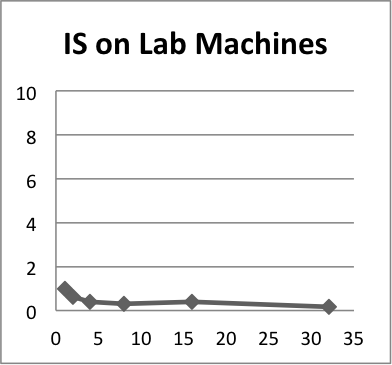
\includegraphics[width=20pc]{Pics-Lab/IS.png}
\end{figure}

\begin{figure}[tbp]
  \centering
  \caption{LU Benchmark on Lab Machines}
	\label{LabLU}
  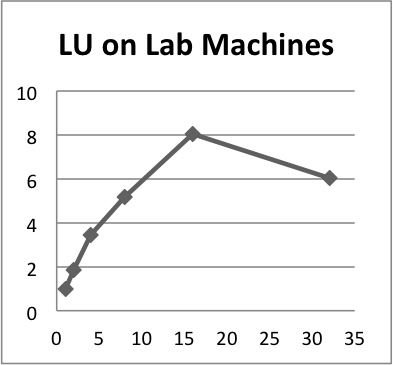
\includegraphics[width=20pc]{Pics-Lab/LU.png}
\end{figure}

\begin{figure}[tbp]
  \centering
  \caption{MG Benchmark on Lab Machines}
	\label{LabMG}
  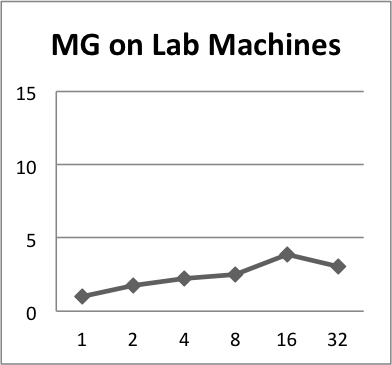
\includegraphics[width=20pc]{Pics-Lab/MG.png}
\end{figure}

\begin{figure}[tbp]
  \centering
  \caption{SP Benchmark on Lab Machines}
	\label{LabSP}
  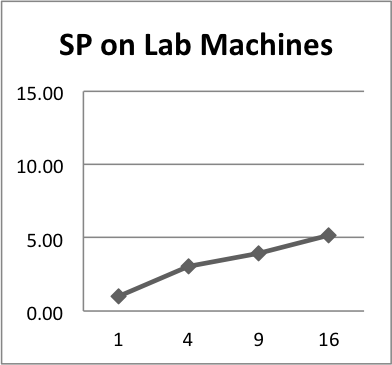
\includegraphics[width=20pc]{Pics-Lab/SP.png}
\end{figure}

\clearpage

%%%%% RASPBERRY PIS %%%%%
\subsection{Raspberry Pis}

%%%%% TABLE %%%%%
Table~\ref{PiTable} shows the Pis' NPB results. The class A benchmarks were used.

\begin{table*}[tbp]
\centering
\caption{Raspberry Pi Benchmark Results}
\label{PiTable}
\begin{tabular}{ c | c || c | c | c | c }
	Benchmark & Nodes & Time & Speedup & MOPS & Process MOPS\\ \hline
    BT & 1 & 4252.40 & 1.00  & 39.57 & 39.57 \\
    BT & 4 & 858.28 & 4.95  & 196.07 & 49.02 \\
    EP & 1 & 334.98 & 1.00  & 1.60   & 1.60 \\
    EP & 2 & 167.65 & 2.00  & 3.20   & 1.60 \\
    EP & 3 & 111.90 & 2.99  & 4.80   & 1.60 \\
    EP & 4 & 84.16 & 3.98  & 6.38  & 1.59 \\
    EP & 5 & 67.38 & 4.97  & 7.97  & 1.59 \\
    FT & 2 & 211.66 & 1.00  & 33.72 & 16.86 \\
    FT & 4 & 93.78 & 2.26  & 76.10  & 19.02 \\
    IS & 1 & 24.78 & 1.00  & 3.39  & 3.39 \\
    IS & 2 & 24.99 & 0.99  & 3.36  & 1.68 \\
    IS & 4 & 16.07 & 1.54  & 5.22  & 1.31 \\
    LU & 1 & 2507.90 & 1.00  & 47.57 & 47.57 \\
    LU & 2 & 1297.50 & 1.93  & 91.95 & 45.97 \\
    LU & 4 & 675.59 & 3.71  & 176.58 & 44.15 \\
    MG & 2 & 98.53 & 1.00  & 39.50  & 19.75 \\
    MG & 4 & 40.84 & 2.41  & 95.30  & 23.82 \\
    SP & 1 & 3474.10 & 1.00  & 24.47 & 24.47 \\
    SP & 4 & 938.64 & 3.70  & 90.57 & 22.64 \\
\end{tabular}
\end{table*}

%%%%% FIGURES %%%%%
Figures~\ref{PiBT} through~\ref{PiSP} graph those speedup results.

\begin{figure}[tbp]
  \centering
  \caption{BT Benchmark on Pis}
	\label{PiBT}
  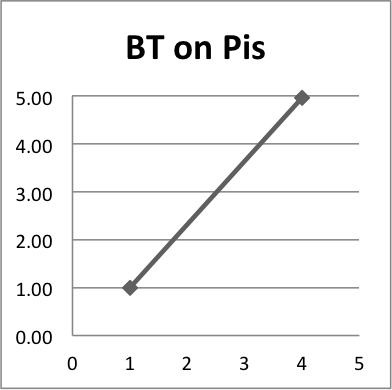
\includegraphics[width=20pc]{Pics-Pi/BT.png}
\end{figure}

\begin{figure}[tbp]
  \centering
  \caption{EP Benchmark on Pis}
	\label{PiEP}
  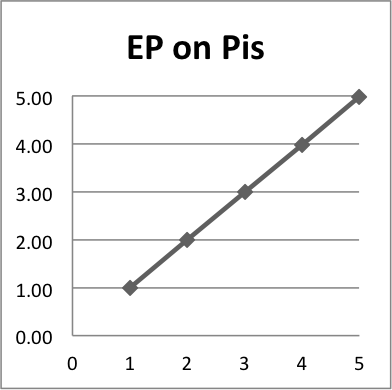
\includegraphics[width=20pc]{Pics-Pi/EP.png}
\end{figure}

\begin{figure}[tbp]
  \centering
  \caption{FT Benchmark on Pis}
	\label{PiFT}
  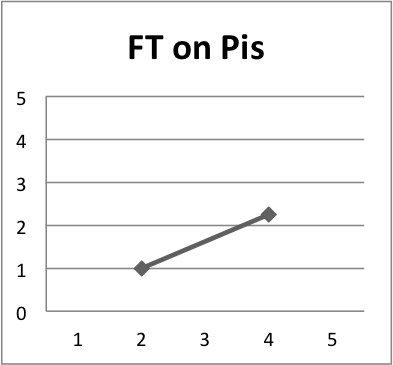
\includegraphics[width=20pc]{Pics-Pi/FT.png}
\end{figure}

\begin{figure}[tbp]
  \centering
  \caption{IS Benchmark on Pis}
	\label{PiIS}
  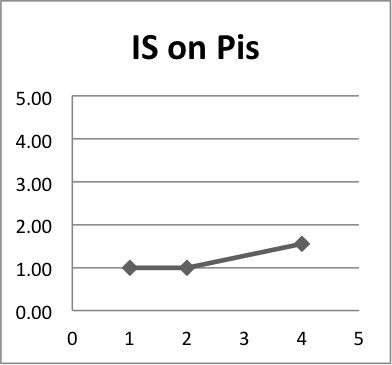
\includegraphics[width=20pc]{Pics-Pi/IS.png}
\end{figure}

\begin{figure}[tbp]
  \centering
  \caption{LU Benchmark on Pis}
	\label{PiLU}
  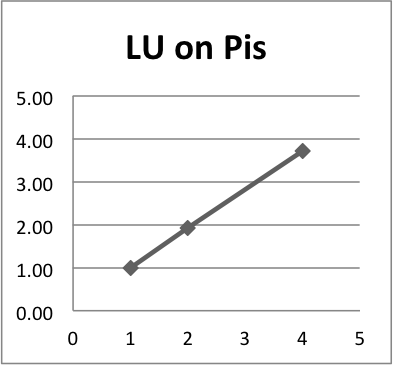
\includegraphics[width=20pc]{Pics-Pi/LU.png}
\end{figure}

\begin{figure}[tbp]
  \centering
  \caption{MG Benchmark on Pis}
	\label{PiMG}
  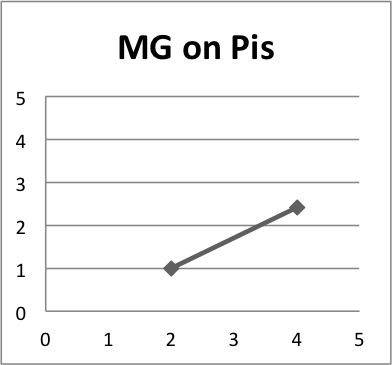
\includegraphics[width=20pc]{Pics-Pi/MG.png}
\end{figure}

\begin{figure}[tbp]
  \centering
  \caption{SP Benchmark on Pis}
	\label{PiSP}
  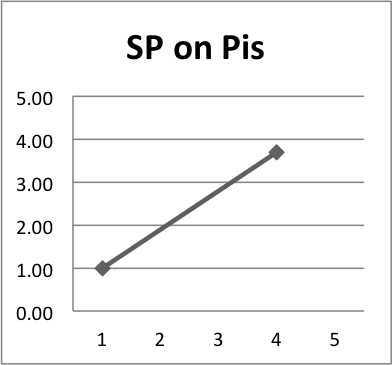
\includegraphics[width=20pc]{Pics-Pi/SP.png}
\end{figure}

\section{Analysis}
Although it's not always the case, we typically notice a linear improvement of runtime when the number of nodes increases. This indicates that the NAS benchmarks, to some extent, can efficiently divide up their work for execution on separate systems, each with their own memory, and then simply combine the results as needed.

Of course, the higher the speedup, the less relient the nodes are on each other. In some cases, we notice that the number of nodes is almost completely tied to the speedup, with perhaps only a small performance hit due to added overhead.

In other situations, there's a very significant performance hit when the workload is distributed (see Figures~\ref{LabIS} and~\ref{PiIS}) and the speedup can even descrease. This happens when the distributed system has to spend more time per node dealing with the extra overhead of initialization and message passing than it spends on the benchmark processing itself.

Figures~\ref{LabLU} and \ref{LabMG} show this as well, but the correlation isn't as clear-cut: using up to 16 nodes improved performance, but past that, performance worsened. This indicates that we should take into account certain thresholds where workload distribution does more harm than good, and the extra nodes would be better used doing other tasks.

In a way, this benchmarking exercise serves to validate distrbuted computing in our eyes. Especially on the Raspberry Pis, despite being somewhat underwhelming individually, we see that having them work together provides a huge increase in performance and that there's real value in using many (potentially unremarkable) systems to process large amounts of data.

\bibliographystyle{abbrv}
%\bibliography{sample}

%\balancecolumns 

\end{document}
